%%%%%%%%%%%%%%%%%%%%%%%%%%%%%%%%%%%%%%%%%%%%%%%%%%%%%%%%%%%%%%%%%%%%%%%%%%%%%%%%
%2345678901234567890123456789012345678901234567890123456789012345678901234567890
%        1         2         3         4         5         6         7         8

\documentclass[letterpaper, 10 pt, conference]{ieeeconf}  % Comment this line out
                                                          % if you need a4paper
%\documentclass[a4paper, 10pt, conference]{ieeeconf}      % Use this line for a4
                                                          % paper

\IEEEoverridecommandlockouts                              % This command is only
                                                          % needed if you want to
                                                          % use the \thanks command
\overrideIEEEmargins
% See the \addtolength command later in the file to balance the column lengths
% on the last page of the document
\usepackage{amssymb,amsmath,graphicx,multicol,bm}
\usepackage[margin=.75in]{geometry}
%\usepackage[mathcal]{euscript}


% The following packages can be found on http:\\www.ctan.org
%\usepackage{graphics} % for pdf, bitmapped graphics files
%\usepackage{epsfig} % for postscript graphics files
%\usepackage{mathptmx} % assumes new font selection scheme installed
%\usepackage{times} % assumes new font selection scheme installed
%\usepackage{amsmath} % assumes amsmath package installed
%\usepackage{amssymb}  % assumes amsmath package installed

\title{\LARGE \bf
Task-Informed Embedded State Transitions for Model-Based Reinforcement Learning
}

%\usepackage{amsthm}
\newtheorem{prop}{Proposition}

%\author{ \parbox{3 in}{\centering Huibert Kwakernaak*
%         \thanks{*Use the $\backslash$thanks command to put information here}\\
%         Faculty of Electrical Engineering, Mathematics and Computer Science\\
%         University of Twente\\
%         7500 AE Enschede, The Netherlands\\
%         {\tt\small h.kwakernaak@autsubmit.com}}
%         \hspace*{ 0.5 in}
%         \parbox{3 in}{ \centering Pradeep Misra**
%         \thanks{**The footnote marks may be inserted manually}\\
%        Department of Electrical Engineering \\
%         Wright State University\\
%         Dayton, OH 45435, USA\\
%         {\tt\small pmisra@cs.wright.edu}}
%}

\author{Ryan Theisen}%$^{1}$% <-this % stops a space
%\thanks{$^{1}$Arizona State University, ryan.theisen@asu.edu}}


\begin{document}



\maketitle
\thispagestyle{empty}
\pagestyle{empty}


%%%%%%%%%%%%%%%%%%%%%%%%%%%%%%%%%%%%%%%%%%%%%%%%%%%%%%%%%%%%%%%%%%%%%%%%%%%%%%%%
\begin{abstract}

We explore a technique to model state transitions for use in model-based reinforcement learning. We use a latent encoding of the state space to 1) model a transition distribution between states conditioned on actions and 2) predict a distribution over rewards given a transition realization. We show that, in addition to being used in a fully model based setting, this method can be used to augment a variety of different reinforcement learning techniques.

\end{abstract}


%%%%%%%%%%%%%%%%%%%%%%%%%%%%%%%%%%%%%%%%%%%%%%%%%%%%%%%%%%%%%%%%%%%%%%%%%%%%%%%%
\section{INTRODUCTION}

In model based reinforcement learning (RL), the representative agent is assumed to have full knowledge of the state-transition distribution $p(s'|s,a)$. For example, in Q-learning, the agent can learn the optimal policy $\pi$ by iteratively applying the Bellman backup equation:
\begin{align*}
	Q(s,a) = R(s) + \gamma\mathbb{E}_{s'\sim p(s'|s,a)}[\text{argmax}_{a'}Q(s',a')]
\end{align*}
where $\pi(s) = \text{argmax}_{a}Q(s,a)$. However, in most real-world cases, the state transition dynamics are unknown, leading to alternate approaches to the RL problem, which are unable to make use of the information provided by $p(s'|s,a)$.

We propose a new method for estimating the state transition distribution, except defining the transition instead on a latent representation $z\in\mathcal{Z}$ of the actual state $s\in\mathcal{S}$. Approaches to encoding input in such a way have been widely studied in the machine learning literature, and have been shown to be useful estimators of the latent data manifold. For examples, in variational autoencoders (VAEs), the latent distribution $p(z|x)$ is derived by minimizing a variation lower bound of the data likelihood. We employ a similar approach to encode the state $s$ into a latent distribution $p(z|s)$, which is in turn used to estimate a distribution $p(z'|z,a)$ that approximates the transition dynamics $p(s'|s,a)$. Furthermore, we model the reward received after transitioning to a new state as a distribution $p(r|z')$.

\section{BACKGROUND}
*to do*

\section{TASK-INFORMED EMBEDDED STATE TRANSITIONS}

\subsection{General Method}
%Consider the problem of representing the state $s\in\mathcal{S}$ by a probability distribution over a latent encoding, $p(z|s)$. Two desirable properties for such a representation to have are \textit{sufficiency} and \textit{minimality}. One says that a representation $z$ is \textit{sufficient} for a task $y$ if $I(y;s) = I(y;z)$. A representation $z$ of the state $s$ is \textit{minimal} if $I(s;z)$ is a small as possible while satisfying sufficiency. In particular, in this work, we consider the task of estimating the transition probability from a latent state $z \in \mathcal{Z}$ into another state $z'\in\mathcal{Z}$ after conditioning on an action $a\in\mathcal{A}$. In this case, the sufficiency condition is reduced to minimizing the conditional entropy $H(s'|z')$ and $H(z'|z)$; that is, we would like $z'$ to encode as much information about the state as possible and similarly that $z$ encode as much information about the transition to $z'$ as possible.

%Furthermore, we would like that our representations $z$ and $z'$ are jointly minimal; that is, $I(s;z), I(z;z')$ are as small as possible given (1)-(2) hold. (Achille and Soatto 2017) showed that the Information Bottleneck (IB) Lagrangian (Tibshy et al)
%\begin{align*}
%\mathcal{L}(\theta) = \eta_1H(s'|z') + \eta_2 H(z'|z) + \beta_1I(s;z) + \beta_2I(z;z')
%\end{align*}
%yields representations that are both sufficient and minimal. 
Consider the common task of modeling an observed variable $X$ in terms of a latent representation $Z$. There are many ways to characterize what properties such a representation should have, though a reasonable approach, and the one we employ in this paper, is defined by the notions of \textit{sufficiency} and \textit{minimality}. Sufficiency, in particular, is relative to a particular task; that is, for a given task $Y$, the representation $Z$ should encode all the necessary information about $X$ to accomplish $Y$. We can express this formally in terms of mutual information via the condition: $I(X;Y) = I(Z;Y)$. Minimality, in turn, means that $Z$ should contain as little information from $X$ as possible while be sufficient for the given task. Formally, we would like that $I(X;Z)$ is a small as possible while having $Z$ be sufficient. Noting that $I(X;Y) - I(Z;Y) = H(Y|Z) - H(Y|X)$, we can write this in terms of a constrained optimization problem:
\begin{align*}
\text{minimize  }& I(X;Z)\\
\text{s.t.  }& H(Y|X) = H(Y|Z)
\end{align*}
Such an objective has been studied previously in the literature (Achille, Soatto 2017; Tibshy 2015), and is known as the Information Bottleneck Principal, with the associated objective:
\begin{align*}
\mathcal{L} = H(Y|Z) + \beta I(X;Z)
\end{align*}
In this paper, we study a particular case of this problem, where the task is twofold: (i) recovering the reward $r$ and (ii) modeling the transition dynamics $p(s'|s,a)$.

Ignoring task (ii) for the moment, we see task (i) is a straightforward example of the above objective, in which we have:
\begin{align*}
\mathcal{L} = H(r|z) + \beta I(s;z)
\end{align*}

To consider task (ii), we first consider a sample trajectory $(s, a, s', r)$, in particular noting that $s' \sim p(s' | s,a)$. We would like to have an encoding $p(z'|z,a)$ that models this distribution as closely as possible. In particular, we consider the following addition to the above objective:
\begin{align*}
 D_{KL}(p(z'|s') \| p(z'|z,a))
\end{align*}
That is, the latent transition distribution for the next state given the current state and $a\in\mathcal{A}$ should "look like" the latent distribution for the next state (which is by nature conditioned on the previous state and action). Then we define the aggregate objective as follows:
\begin{align*}
\mathcal{L} = H(r|z') + \beta I(s;z) + \lambda D_{KL}(p(z'|s') \| p(z'|z,a))
\end{align*}
Note that the encodings $p(z'|s')$ and $p(z|s)$ share the same generating function (a neural network), simply conditioned on different states. See Figure 1 for a diagram of the final model.

\begin{figure}[t]
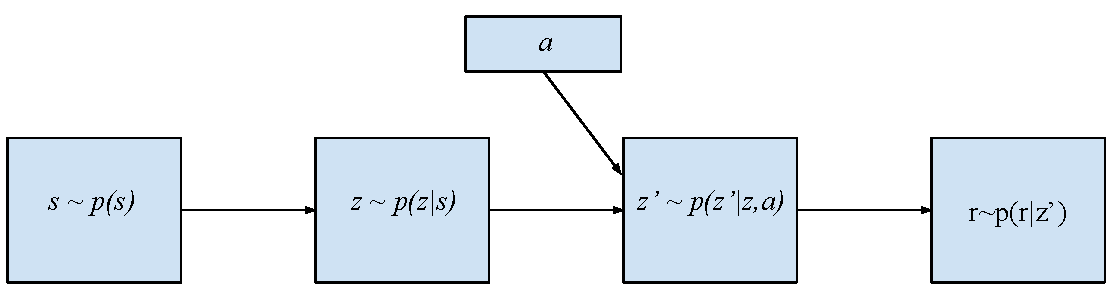
\includegraphics[width=8cm]{latentTransitionModel.pdf}
\caption{A diagram of the latent transition model. In practice, the encoder $p(z|s)$, transition $p(z'|z,a)$, and reward $p(r|z')$ are parameterized as neural networks that output the parameters of some distribution (e.g. a Gaussian).}
\centering
\end{figure}


\section{EXAMPLE: MODEL-BASED Q-LEARNING}

\subsection{Monte Carlo Model-Based Q Learning}
Consider the standard Bellman Equation:
\begin{align*}
	Q(s,a) = R(s) + \gamma\mathbb{E}_{s'\sim p(s'|s,a)}[\text{argmax}_{a'}Q(s',a')]
\end{align*}
Under the hypothesis that the representation $z$ is sufficient for the given task, we can reframe this problem in terms of the latent encoding $z$:
\begin{align*}
	Q(z,a) &= R(z) + \gamma\mathbb{E}_{z'\sim p(z'|z,a)}[\text{argmax}_{a'}Q(z',a')]\\
	&= R(z) + \gamma\int_\mathcal{Z} \text{argmax}_{a'}Q(z',a')p(z'|z,a)dz'
\end{align*}
Since $p(z'|z,a)$ is known, we can estimate this integral using a Monte Carlo approach:
\begin{align*}
	Q(z,a) &= R(z) + \gamma\int_\mathcal{Z} \text{argmax}_{a'}Q(z',a')p(z'|z,a)dz'\\
	&\approx R(z) + \frac{\gamma}{N}\sum_{k=1}^N \text{argmax}_{a'}Q(z_k',a')
\end{align*}
where $z'_1,...,z'_N \sim p(z'|z,a)$ and $R(z) \sim p(r|z)$.

Using this set up, we can estimate $Q$ using a modified version of the DQN algorithm, minimizing the objective
\begin{align*}
	\mathcal{L} = \frac{1}{2}\Big(Q(z,a)-\big(R(z) + \frac{\gamma}{N}\sum_{k=1}^N \text{argmax}_{a'}Q(z_k',a')\big)\Big)^2 
\end{align*}
Note that, unlike the standard DQN algorithm, given the distribution $p(z'|z,a)$ and the function $R(z)$, this formulation can be trained entirely off-line, with no active interaction with the environment.

\section{EXPERIMENTS}

\section{CONCLUSION AND FUTURE WORK}










\end{document}
